\chapter{Implementation} \label{cpt-implementation}

The implementation used for the experiment is based on an implementation within the framework \emph{Diligent Engine} 
\cite{DiligentGraphicsGitHub, DiligentGraphics}. This framework includes rendering backend supporting 
multiple rendering \ac{API}s, with modern integrations for \ac{GPU}-driven rendering. One of these modern 
features is the support for mesh shading in Microsoft's D3D12 rendering \ac{API}. The support for modern 
rendering features, while still maintaining access to all core features, makes \emph{Diligent Engine} a good 
place to start from. For the experiment, the Mesh Shading pipeline is enhanced to better fit purpose of drawing 
a huge amount of voxels. Also, the integrated view-frustum culling was altered to some degree so that it works on 
meshlet-groups rather than meshlets themselves. This change was made during the restructuring of the draw tasks. 
The updated pipeline changes how meshes are dispatched because of the use of additional acceleration structures. 
This chapter provides an overview of all the changes and additions to the framework and how the pipeline works 
in particular. The full implementation details can be found in the appendix \ref{cpt-appendix}.

\section{Pipeline Overview} \label{sec-piepline-initialization}

[@TODO: Add meshlet based view frustum culling impl is used and was already in Diligent Engine]

\subsection*{Pipeline Initialization} \label{subsec-piepline-initialization}

\begin{figure}[h]
    \centering
    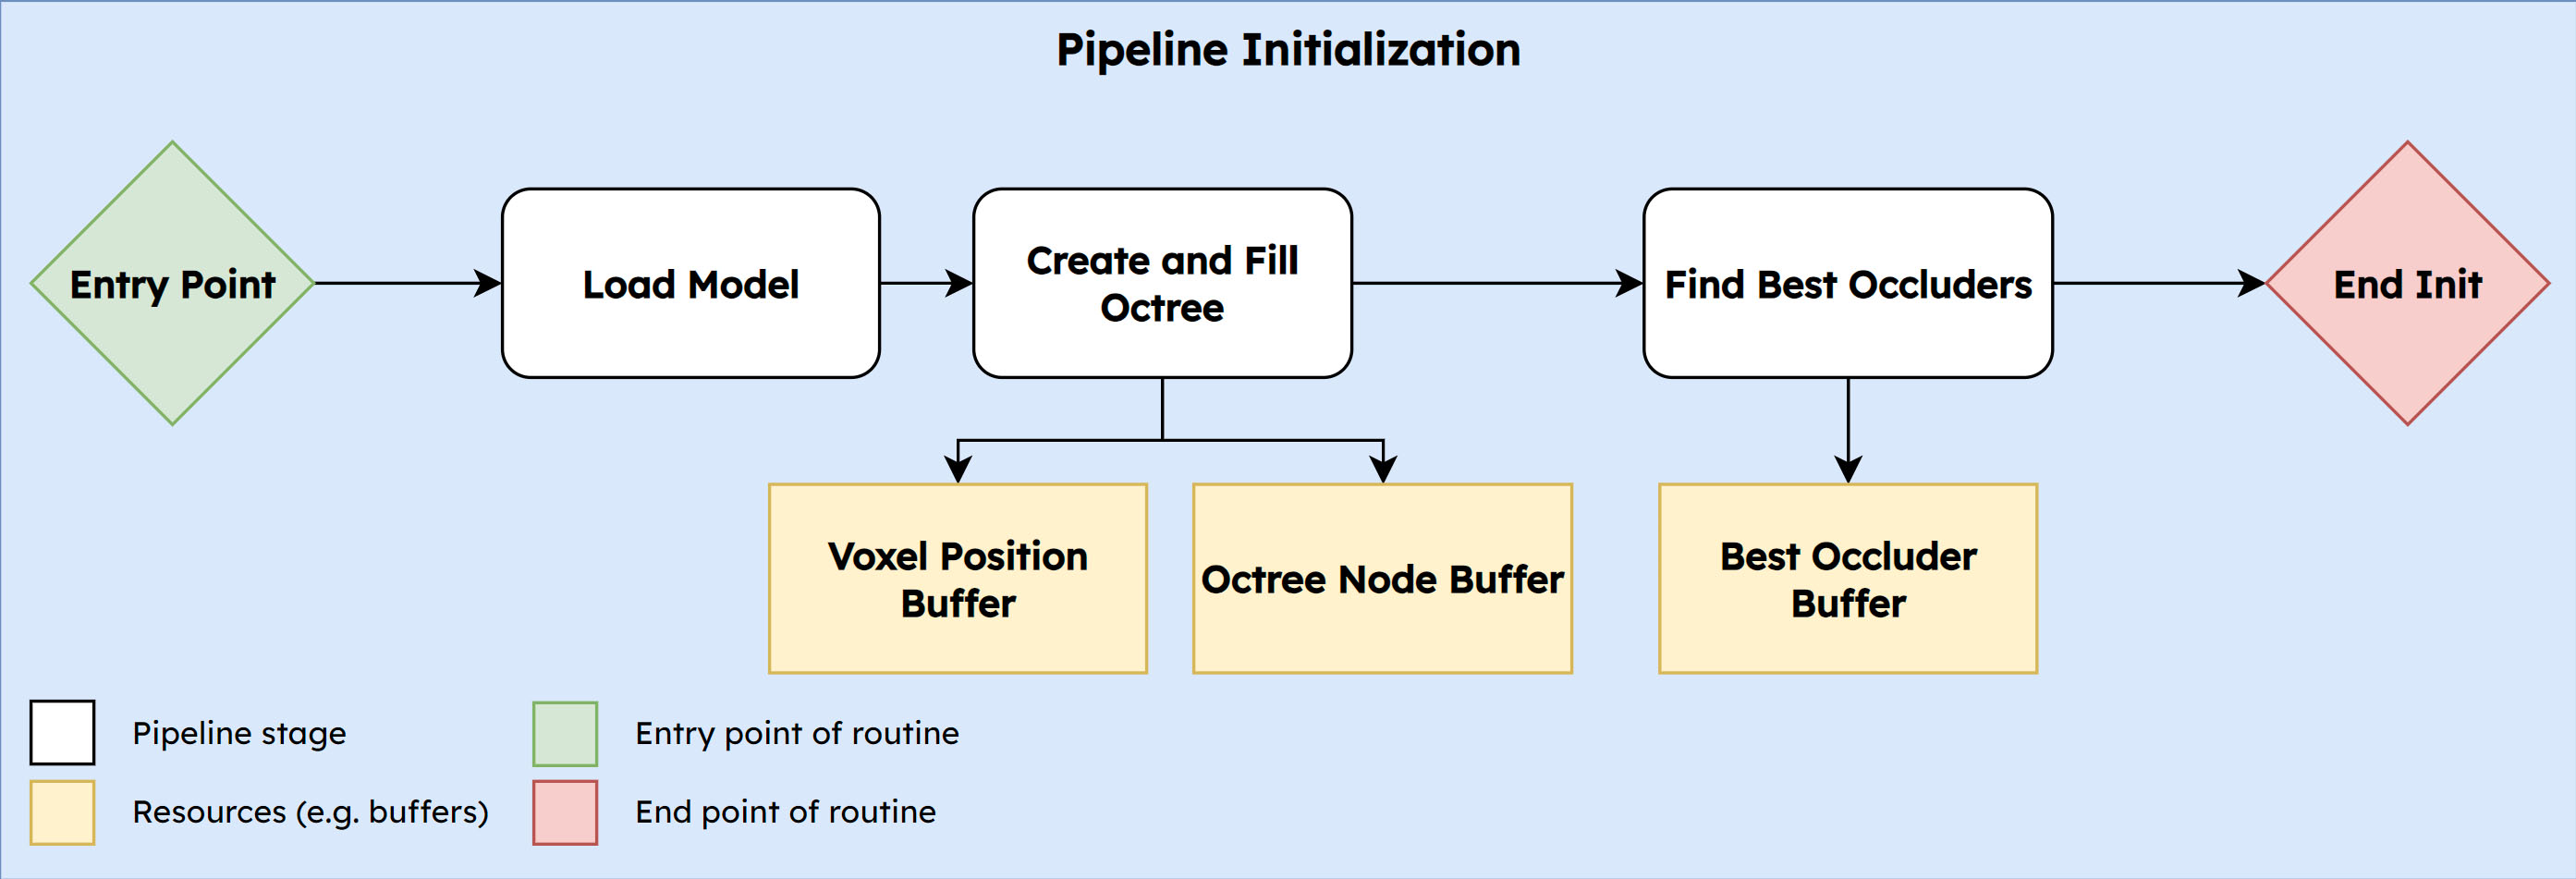
\includegraphics[width=\linewidth]{images/graphics/pipeline-initialization.jpg}
    \caption{The initialization process of the rendering pipeline. Depending on the voxel model, an octree node 
    can hold anything between zero and \emph{n} voxels, \emph{n} being the amount of threads per threadgroup.}
    \label{fig:pipeline-initialization}
\end{figure}

\noindent
The pipeline is, as usual, split into an initialization routine and an update loop. The initialization is 
called once during the beginning of the execution flow and the render loop is initiated after the initialization 
finished. Then, the loop is continuously called - once per frame. Figure \ref{fig:pipeline-initialization} shows 
the initialization procedure. 

\subsubsection*{Voxel Model Loading} \label{subsec-voxel-model-loading}

For the purpose of this experiment, a single, solid voxel mesh is loaded, but this could also be a scene 
consisting of multiple solid voxel models. In the provided implementation, the positions of voxels inside a regular 
grid are loaded, skipping grid cells, where no voxels are located. For loading the voxels, the tool \emph{binvox} 
is used \cite{binvox, Nooruddin2003}. 


\subsubsection*{Octree Creation} \label{subsec-octree-creation}

After loading any voxel model, an octree is created that covers the complete scene - in this case, since there is 
only one model present, the octree's bounding volume is the bouding volume of the voxel model. As discussed in 
chapter \ref{subsec-highres-svo-dags}, it is recommended to use a highly efficient and compressed octree implementation 
like an \ac{SVO} or a Sparse Voxel \ac{DAG} \cite{Kampe2013}. For the purpose of this work, a custom octree 
implementation is used, which refers to indices in a global \emph{voxel position buffer}, as shown in figure 
\ref{fig:voxelpos-octreenode-buffer}.\\

\begin{figure}[h]
    \centering
    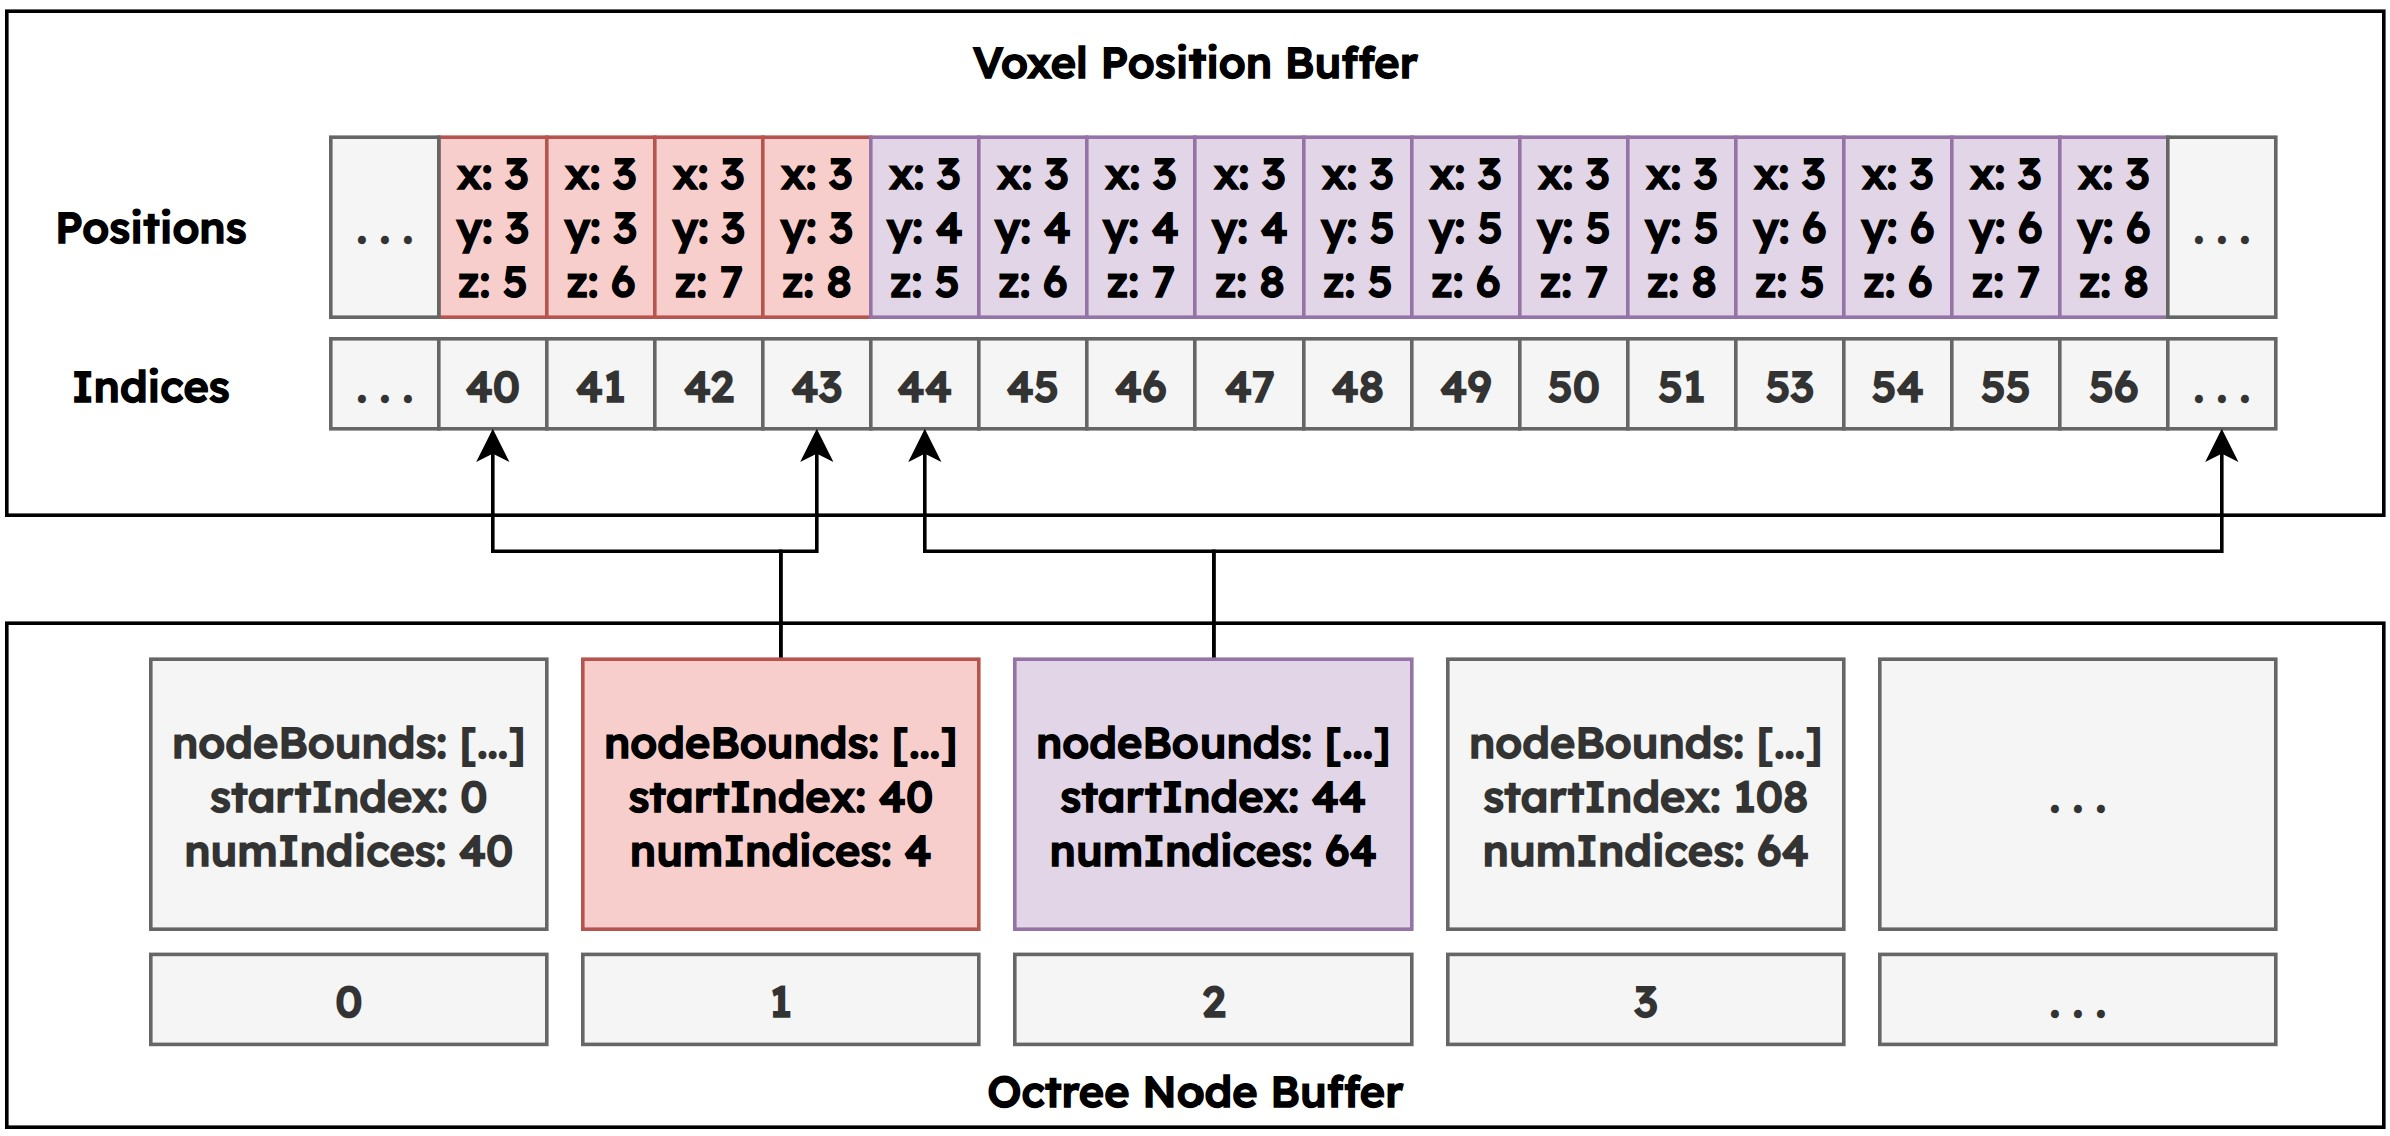
\includegraphics[width=\linewidth]{images/graphics/voxelpos-octreenode-buffer.jpg}
    \caption{The voxel position buffer and the octree node buffer. The latter one providing a 
    specific structure to the first one.}
    \label{fig:voxelpos-octreenode-buffer}
\end{figure}

\noindent
Since the \ac{GPU} is supposed to generate a lot of voxels on the fly, data buffers like the voxel position buffer 
need to be considered.
For structuring the data, various options are available. The initial idea was to lay out the voxels as individual 
meshlets. This means that individual voxels can be culled and each \ac{GPU} thread generates one voxel. This would 
mean that only the voxel position buffer is needed. The task shader takes the positions, culls meshlets 
against the view frustum and dispatches the mesh shader with the given data. As long as no spatial container like 
an octree is used, this approach works fine. When considering the use of an octree, however, another layout serves 
better. In this case, each \ac{GPU} threadgroup takes care of one octree node, with the maximum amount of voxels 
per node being equal to the amount of threads per threadgroup. Using this layout, each thread in a threadgroup 
again takes care of at most one voxel. The octree node information can now store additional information, which can 
be used for octree node based view frustum culling. To generate this data, the octree is queried during the 
initialization, resulting in an extra \emph{octree node buffer} which stores an index pointing to the the voxel 
position buffer and a count of voxels, associated with the node. After sorting the voxel position buffer, this 
additional structure identifies voxel positions that are located adjacent to each other inside an octree node. Figure 
\ref{fig:voxelpos-octreenode-buffer} shows the data layout and how it relates to the voxel position buffer. 


\subsubsection*{Best Occluder Selection} \label{subsec-best-occluder-selection}

The next step in the initialization procedure is to pre-compute the best occluders. This part is a significant one, 
since it computes important data for the occlusion culling. As mentioned in chapter \ref{subsubsec-two-pass-occlusion-culling},
best occluders are usually specifically authored by artists during the creation of the scene. This process is only 
possible, if the models are static in a sense, that they do not change in size or shape. An alteration like this 
could result in inefficient occlusion queries or even the elimination of occluders altogether. In the context of 
volumetric scene representations, where voxel models are often a target of manipulation by players or physical 
interactions, a predetermination of best occluders is not possible in the way it is for static models.
This specific scenario is what the given approach aims for, and why the next step in the pipeline pre-processes best 
occluders. Note, that this implementation does not include an update of the best occluders. It only serves as a 
case study of the occlusion culling algorithm. Updating the best occluders when the voxel model is altered, 
needs to be evaluated seperatly, but is considered to be trivial for occasional changes to the mesh. A more 
demanding change to the octree content is given when computing physical interactions within the duration of a frame.
In this case, further tests need to be done to evaluate the impact on performance. \\

\noindent
To find the best occluders, different constraints need to be considered. The provided approach makes use of the inner, 
non-visible voxels, and approximates them using the octree. This means, an octree node is equivalent to a best occluder, 
if:

\begin{itemize}
    \item the maximum number of voxels per octree node is a product of \begin{math}\emph{width} \times \emph{height} \times \emph{depth}\end{math}
    \item the number of voxels present within the node is equal to the maximum number of voxels per octree node,
    \item and the octree node's boundary is equal to the \emph{minimal convex hull} of all voxels within the node.
\end{itemize}

[@TODO: Check, if this can be reduced due to redundancy]

\noindent [@TODO: Fix this sentence]
The first criterium is necessary to allow for a cubical node shape, filled completely with voxels. The maximum number 
of voxels per node must therefore be a product of the width, length and depth of a voxel chunk. This criterium can 
be changed depending on the setup. A cubical octree structure was selected. The number of maximum voxels per octree node 
is therefore a \emph{power of three}.

\noindent
The second criterium makes sure that the node is full. This is essential for this approach [@TODO: Finish sentence]

\noindent
The last criterium avoids full octree nodes which are not tightly filled. It is an intrinsic feature of an octree 
to maintain differently sized nodes. This means that voxels, which are on the surface of a model, can be part of 
a bigger node, which is not subdivided further. Therefore, a bigger node can be filled with the maximum amount of 
voxels, without being tightly filled. The \emph{minimal convex hull} is thus a boundary volume which has the minimum 
volume while still incorporating all voxels.

\noindent
In practice, this means, that best occluders are given, if the octree node is completely, tightly filled 
with voxels. If the octree node, however, is larger than the block defined by the maximum number of voxels 
per node, this block cannot be approximated correctly by the bounds of the node. This property of a best 
occluder is propagated up the tree, as long as all eight child nodes satisfy the requirements of being a 
best occluder. During the depth pre-pass, the best occluders are drawn as "large voxels" which are the size 
of the respective best occluder node. This can be achieved by simply reusing the mesh shader used in the 
normal draw call, and inputting the node's position and bounds. This way, a whole node gets drawn, instead 
of the individual voxels, reducing the computation cost for the best occluders by at least \emph{n} times, 
with \emph{n} being the maximum amount of voxels per node. The best occluders are separatly stored in a 
buffer, so they can be dispatched efficiently. \\

%[@TODO: Add data structure diagram of best occluder buffer]
%[@TODO: add images]

\noindent
This concludes the initialization of the pipeline. When changes are applied to the voxel data, the voxel buffer,
the octree node buffer and the best occluder buffer need to be updated accordingly. Alternatively, the best 
occluders can be implicitly calculated on the basis of the octree node buffer. This would make the best 
occluders buffer redundant but would result in a higher dispatch count with a lot of discarded nodes, 
where the criteria for best occluder are not met. Since all computations are more or less in parallel, this 
will not affect frametimes for a moderate amount of octree nodes. Nevertheless, since only static voxel models with 
no runtime alternation are assumed for this work, a static, pre-calculated buffer for best occluders can be used.

\subsection*{Rendering Loop} \label{sec-rendering-loop}

\begin{figure}[h]
    \centering
    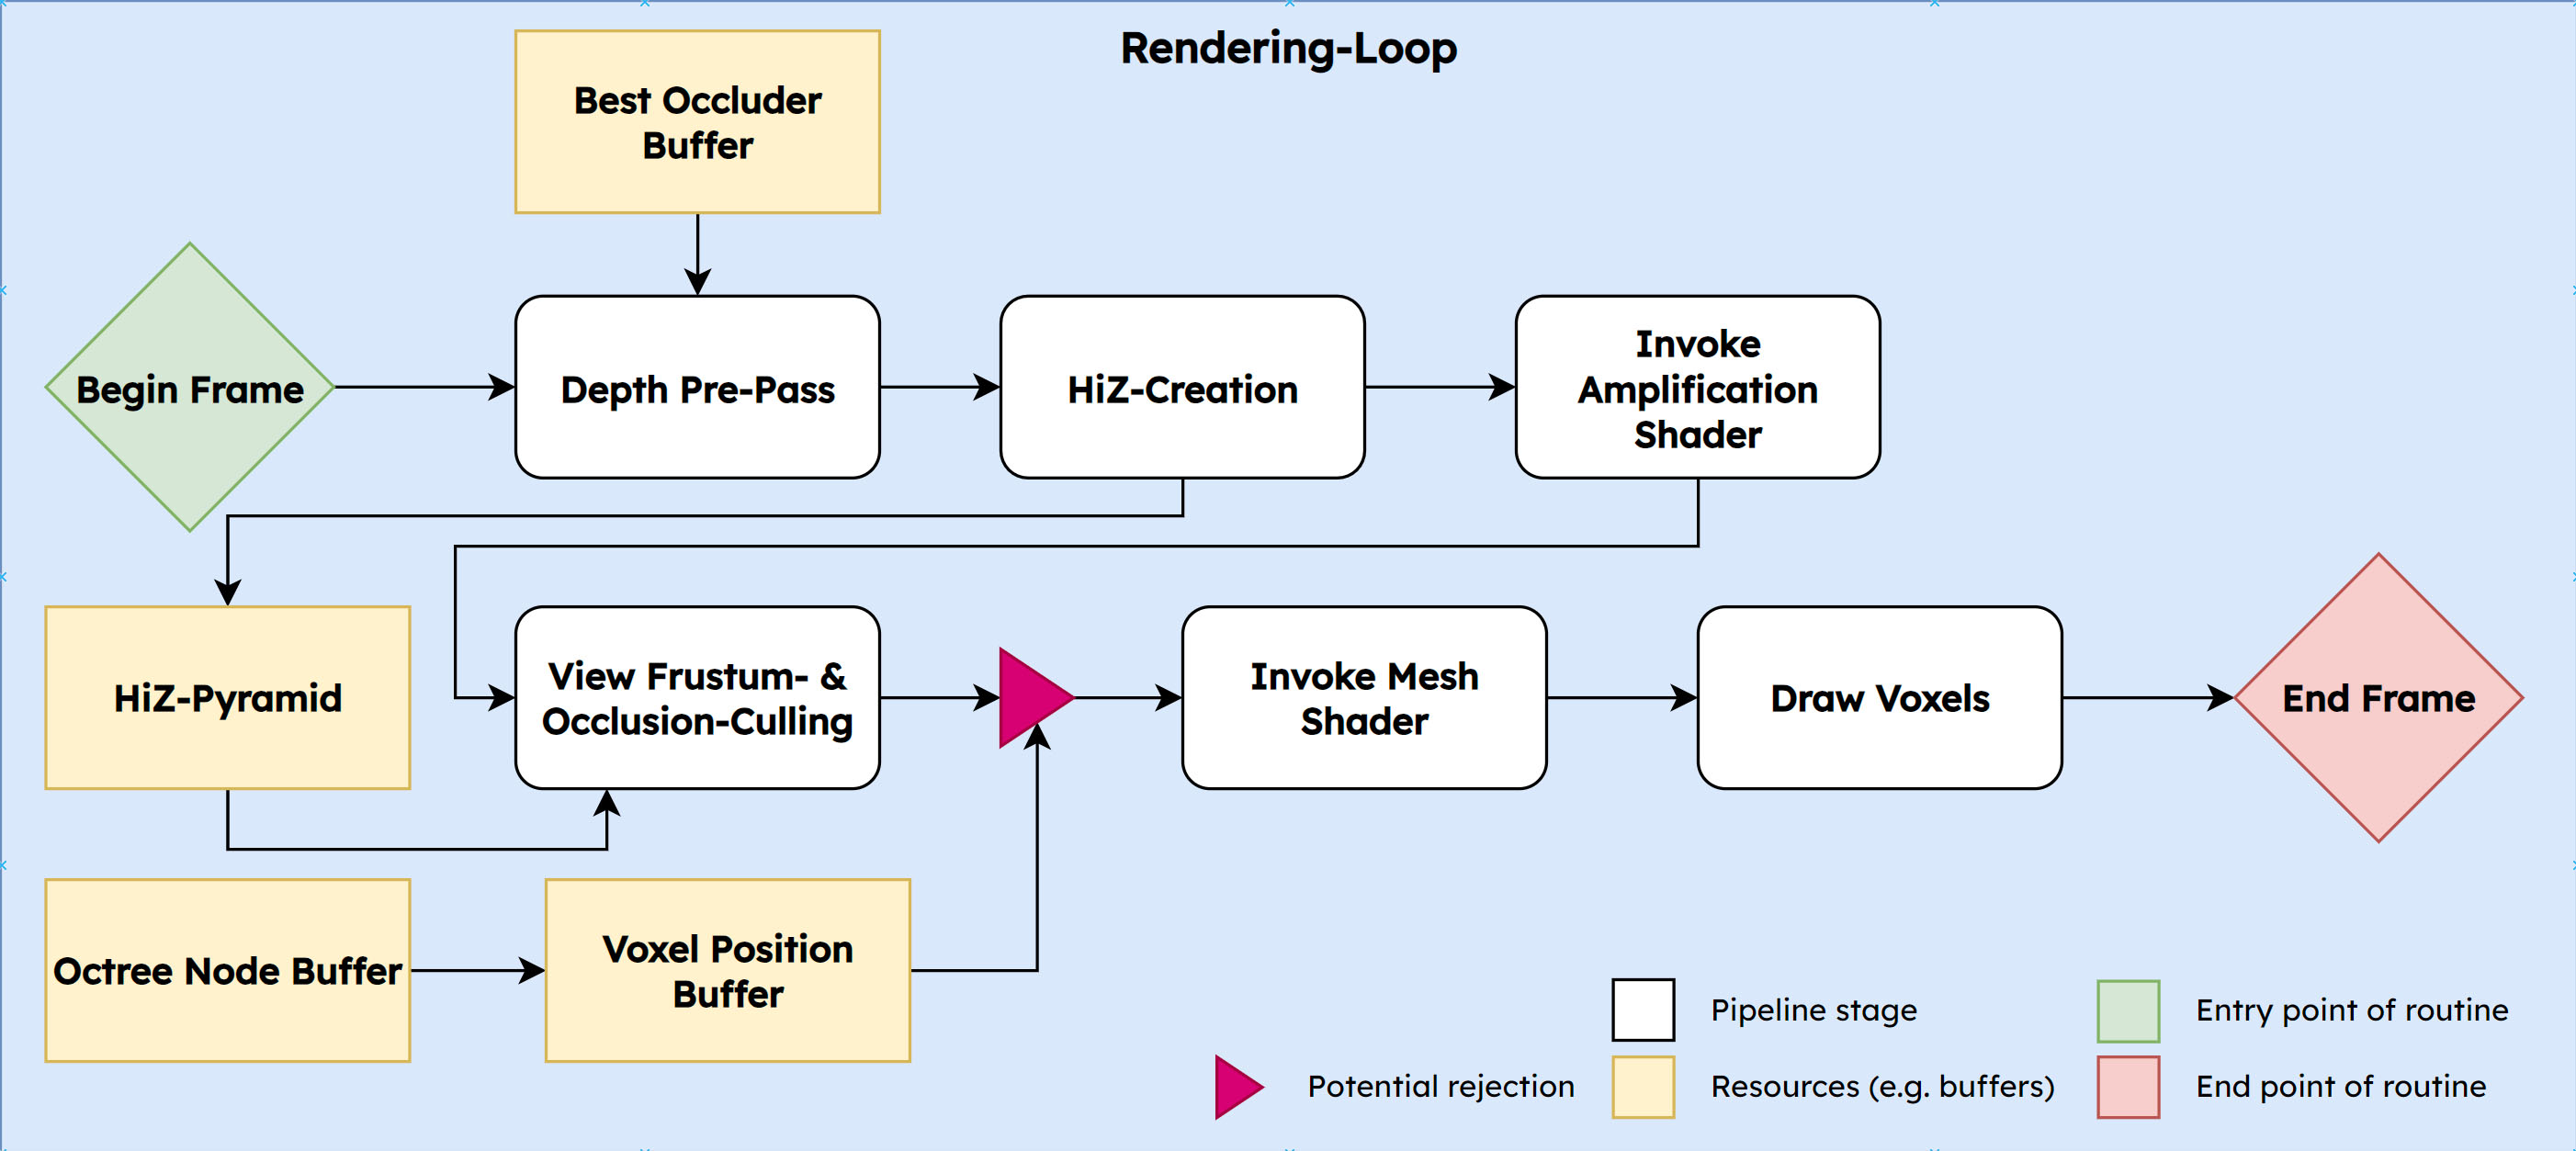
\includegraphics[width=\linewidth]{images/graphics/rendering-loop.jpg}
    \caption{The rendering loop of the rendering pipeline. The red sub-stage of the render loop marks the dispatch 
    of the meshlets, involving the voxel positions and the octree node data. If an octree node or voxel is considered 
    to be culled, the loop ends with the task shader.}
    \label{fig:pipeline-loop}
\end{figure}

\noindent
The rendering loop consists of three main steps: The depth pre-pass including \ac{HiZ} generation, the 
task shader and the mesh shader. The different stages consume and generate various data buffers 
and textures, as shown in figure \ref{fig:pipeline-loop}. 

\subsubsection*{Depth Pre-Pass} \label{subsec-depth-prepass}

The frame computation starts by computing the depth pre-pass, which is the custom render pass central 
to the occlusion culling. In this pass a compute shader is invoked that takes the best occluders and 
draws them to the depth buffer. This depth pass does not draw to the back buffer, making the computation 
relatively efficient. It can also include optional computations like frustum culling for further 
optimization. This can be effective when there are a lot of nodes in the best occluders buffer. 
Consequently, the depth buffer has data from possible occluders and the \ac{HiZ} generation is started. 
The z-pyramid is generated by another compute shader, which samples four texels of the input texture 
(the full resolution depth buffer) and outupts the lowest z-value to an output texture (mip level 1). 
This chain of mip-maps is shown as the [@TODO: here is a jump from mip lvl 1 to full z-pyramid!]
\ac{HiZ}-pyramid in figure \ref{fig:pipeline-loop}.


\subsubsection*{The Task Shader} \label{subsec-task-shader}

Now, the task shader is invoked, each threadgroup resembling one octree node. It decides over which 
meshlets are drawn. Here, view frustum culling is applied to a threadgroup and the occlusion culling is 
executed by projecting the bounding box of the meshlets onto the view plane and querying the 
\ac{HiZ}-pyramid for depth values. If the voxel position is found to be visible - or not occluded by 
the best occluders - the position is added to the payload, ready to be drawn by the mesh shader. 


\subsubsection*{The Mesh Shader} \label{subsec-mesh-shader}

The mesh shader executes the appropriate transformations, constructs a uniform voxel around the voxel position 
and outputs the geometry. The voxels in a \ac{GPU}-Driven approach can be completely generated on the \ac{GPU}, 
minimizing the memory bandwidth used per frame. This optimization technique is not only efficient, but also 
trivial for uniform, static voxel geometry. When dispatching one voxel per thread, one voxel corresponds 
to one meshlet, making pre-computation completely redundant, as opposed to the common precomputation of meshlets, 
as mentioned in chapter \ref{sec-mesh-shading}. 


\section{Data Processing} \label{sec-data-flow}

[@TODO: Fix image positions]
To illustrate the pipeline in even more detail, this chapter focuses on the data and how it is sampled, computed 
and output throughout the pipeline.

\subsection*{Data Pre-Processing}

To obtain a valid model for the pipeline, a voxel mesh has to be created. To do this, \emph{binvox} 
\cite{binvox} can be used. It works with any triangle mesh in the \emph{.obj} (Wavefront) or \emph{.ply} 
(Stanford Polygon File Format) format, which in turn can be exported by most of the common 3D software. 
Due to its availability, \emph{Blender} \cite{Blender} is recommended. To convert the triangle mesh to a volumetric 
voxel representation, \emph{binvox} is executed from the command line and the input file as well as optional 
parameters are specified. The output is a \emph{.binvox} file. Figure \ref{fig:trimesh-to-voxel-mesh} shows 
both the triangle mesh and the processed volumetric voxel mesh. 

\begin{figure}[h]
    \centering
    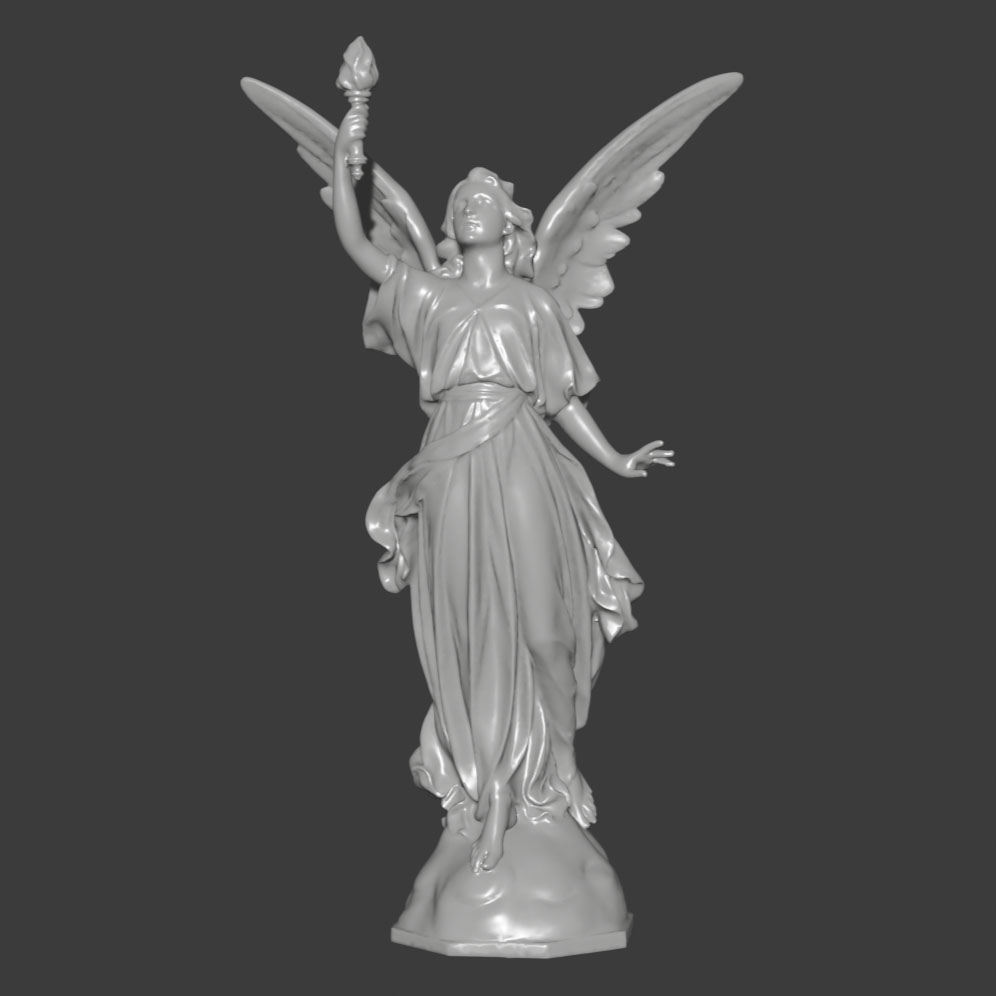
\includegraphics[width=200px]{images/graphics/lucy-triangle-mesh.jpg}
    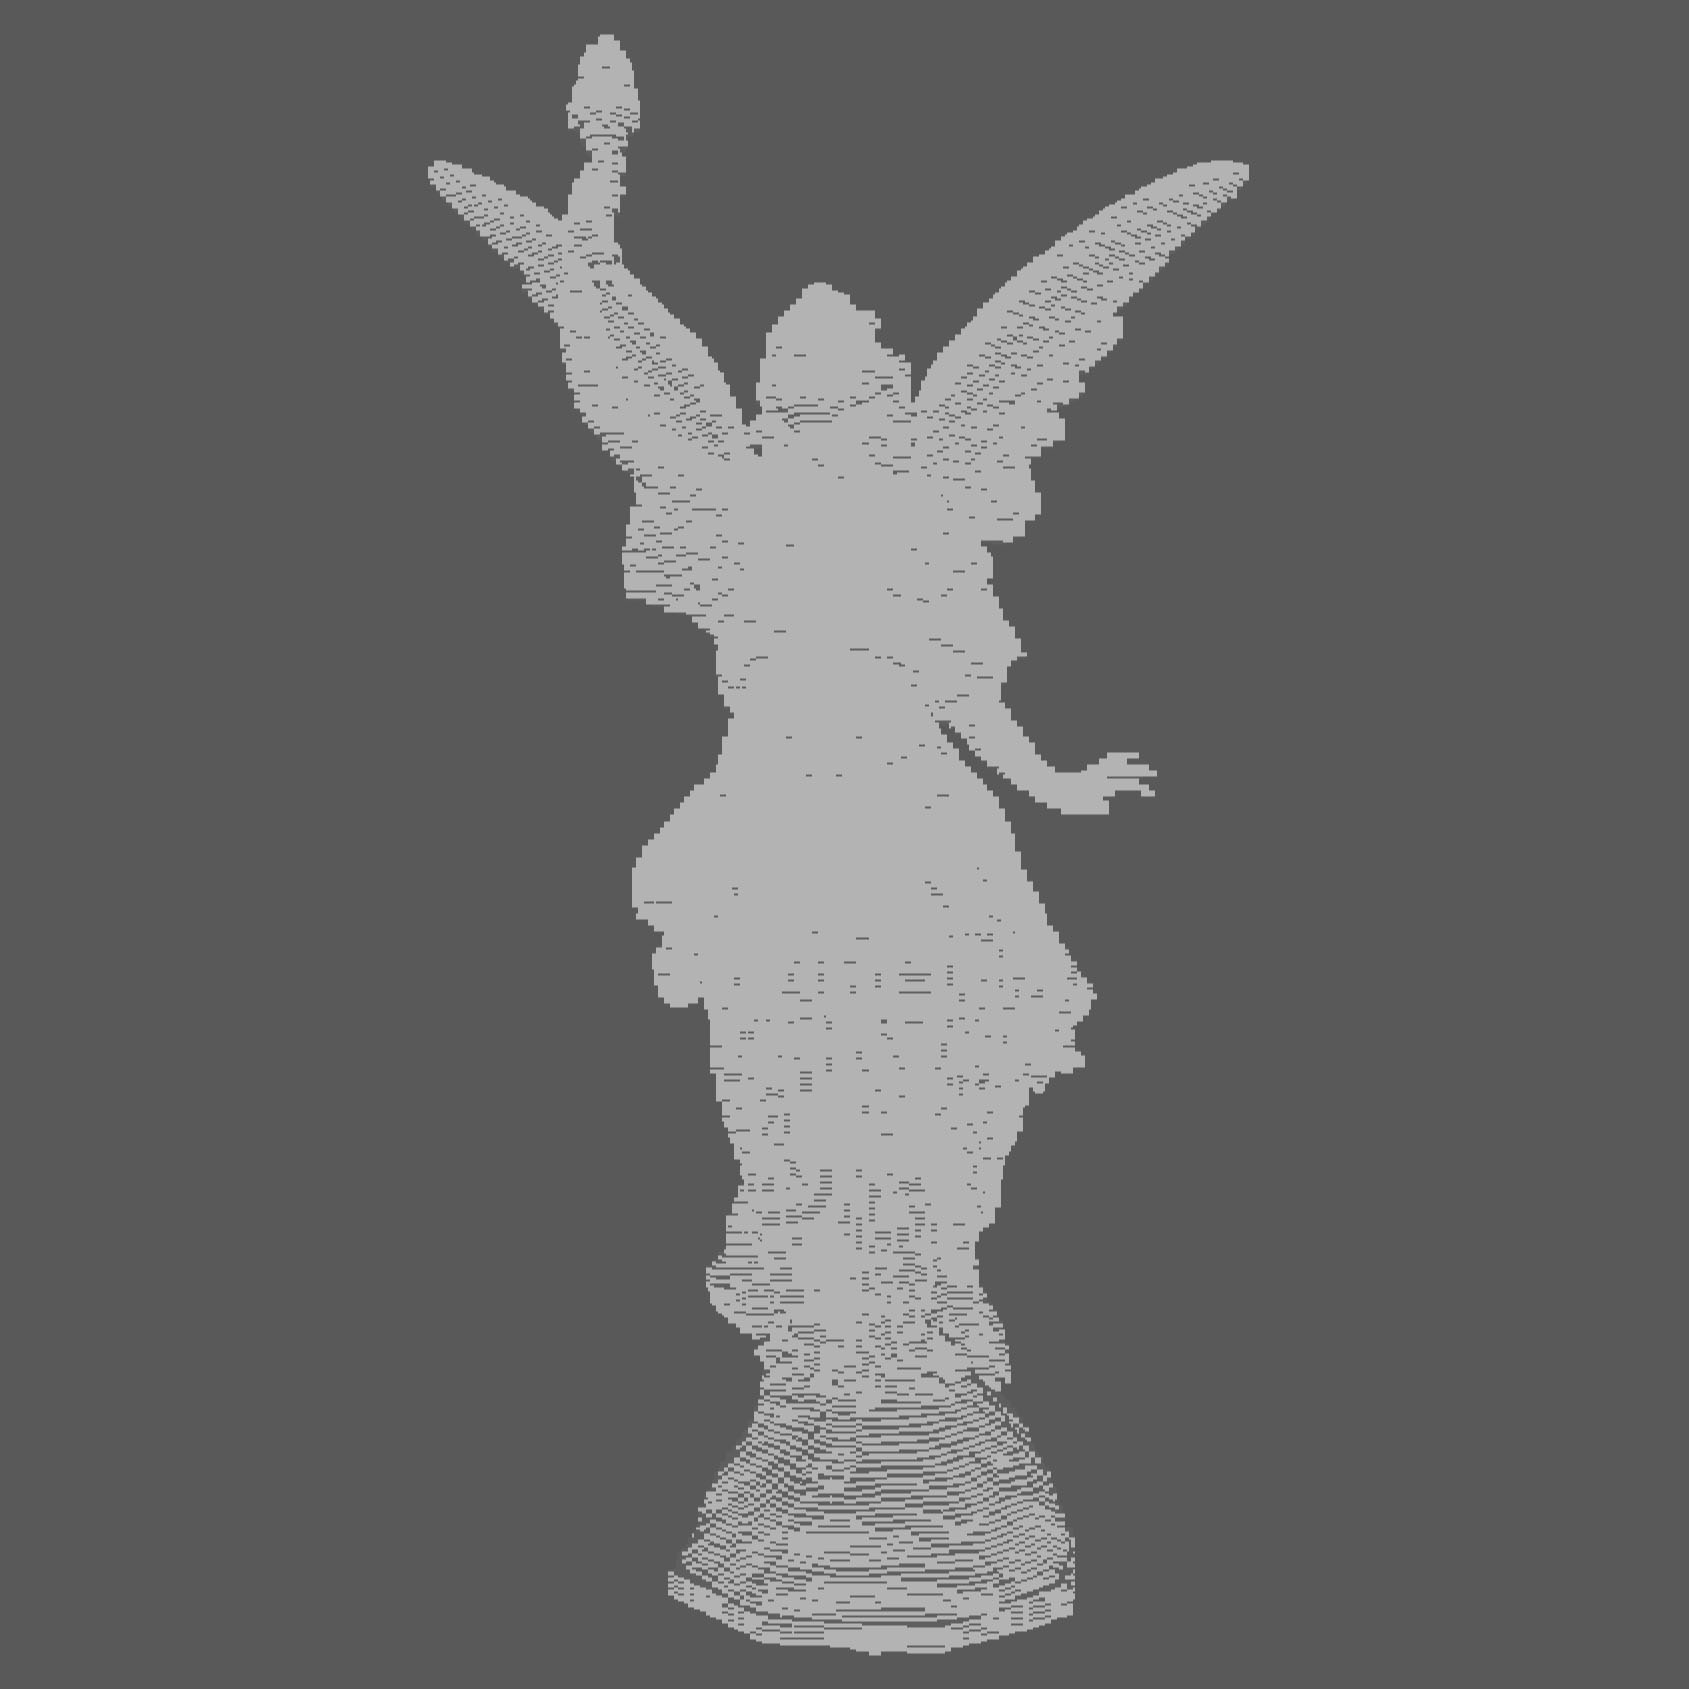
\includegraphics[width=200px]{images/graphics/lucy-voxel-mesh.jpg}
    \caption{The input triangle mesh (left) and the voxelized and parsed voxel mesh (right). 
    Model \emph{Lucy} from \emph{The Stanford 3D Scanning Repository} \cite{Stanford23}.}
    \label{fig:trimesh-to-voxel-mesh}
\end{figure}

\noindent
The engine then takes the \emph{.binvox} file as an input and loads it during initialization. This data is then
parsed, ready to be input into the octree.


\subsection*{Octree Generation}

The octree implementation allows for a \emph{boundary} and a \emph{maximum instances per node threshold} to be defined. 
The boundary defines the space, which the octree occupies in the scene. All instances added to the octree must 
be located within this boundary. Otherwise the octree cannot resolve the instance spatially. The maximum threshold 
of instances is checked whenever an instance is added to the octree. If the maximum is exceeded, the node is split into 
child nodes, which are then filled with the node's data. The loaded voxel model is located in a regular 
grid, which can be used to calculate the bounds of the octree. Each voxel is then added to the octree, which 
automatically divides the space according to the voxel density, always satisfying the constraint of the maximum 
amount of voxels per node. Figure \ref{fig:voxel-octree-viz} shows that the voxels are grouped into octree nodes. 
The octree can be queried with a reference to an output buffer. This buffer is then filled with the lightweight octree 
node structure, for the \ac{GPU} to consume. Empty nodes are not added to the buffer, hence the name \emph{Sparse 
Voxel Octree}. 


\begin{figure}[h]
    \centering
    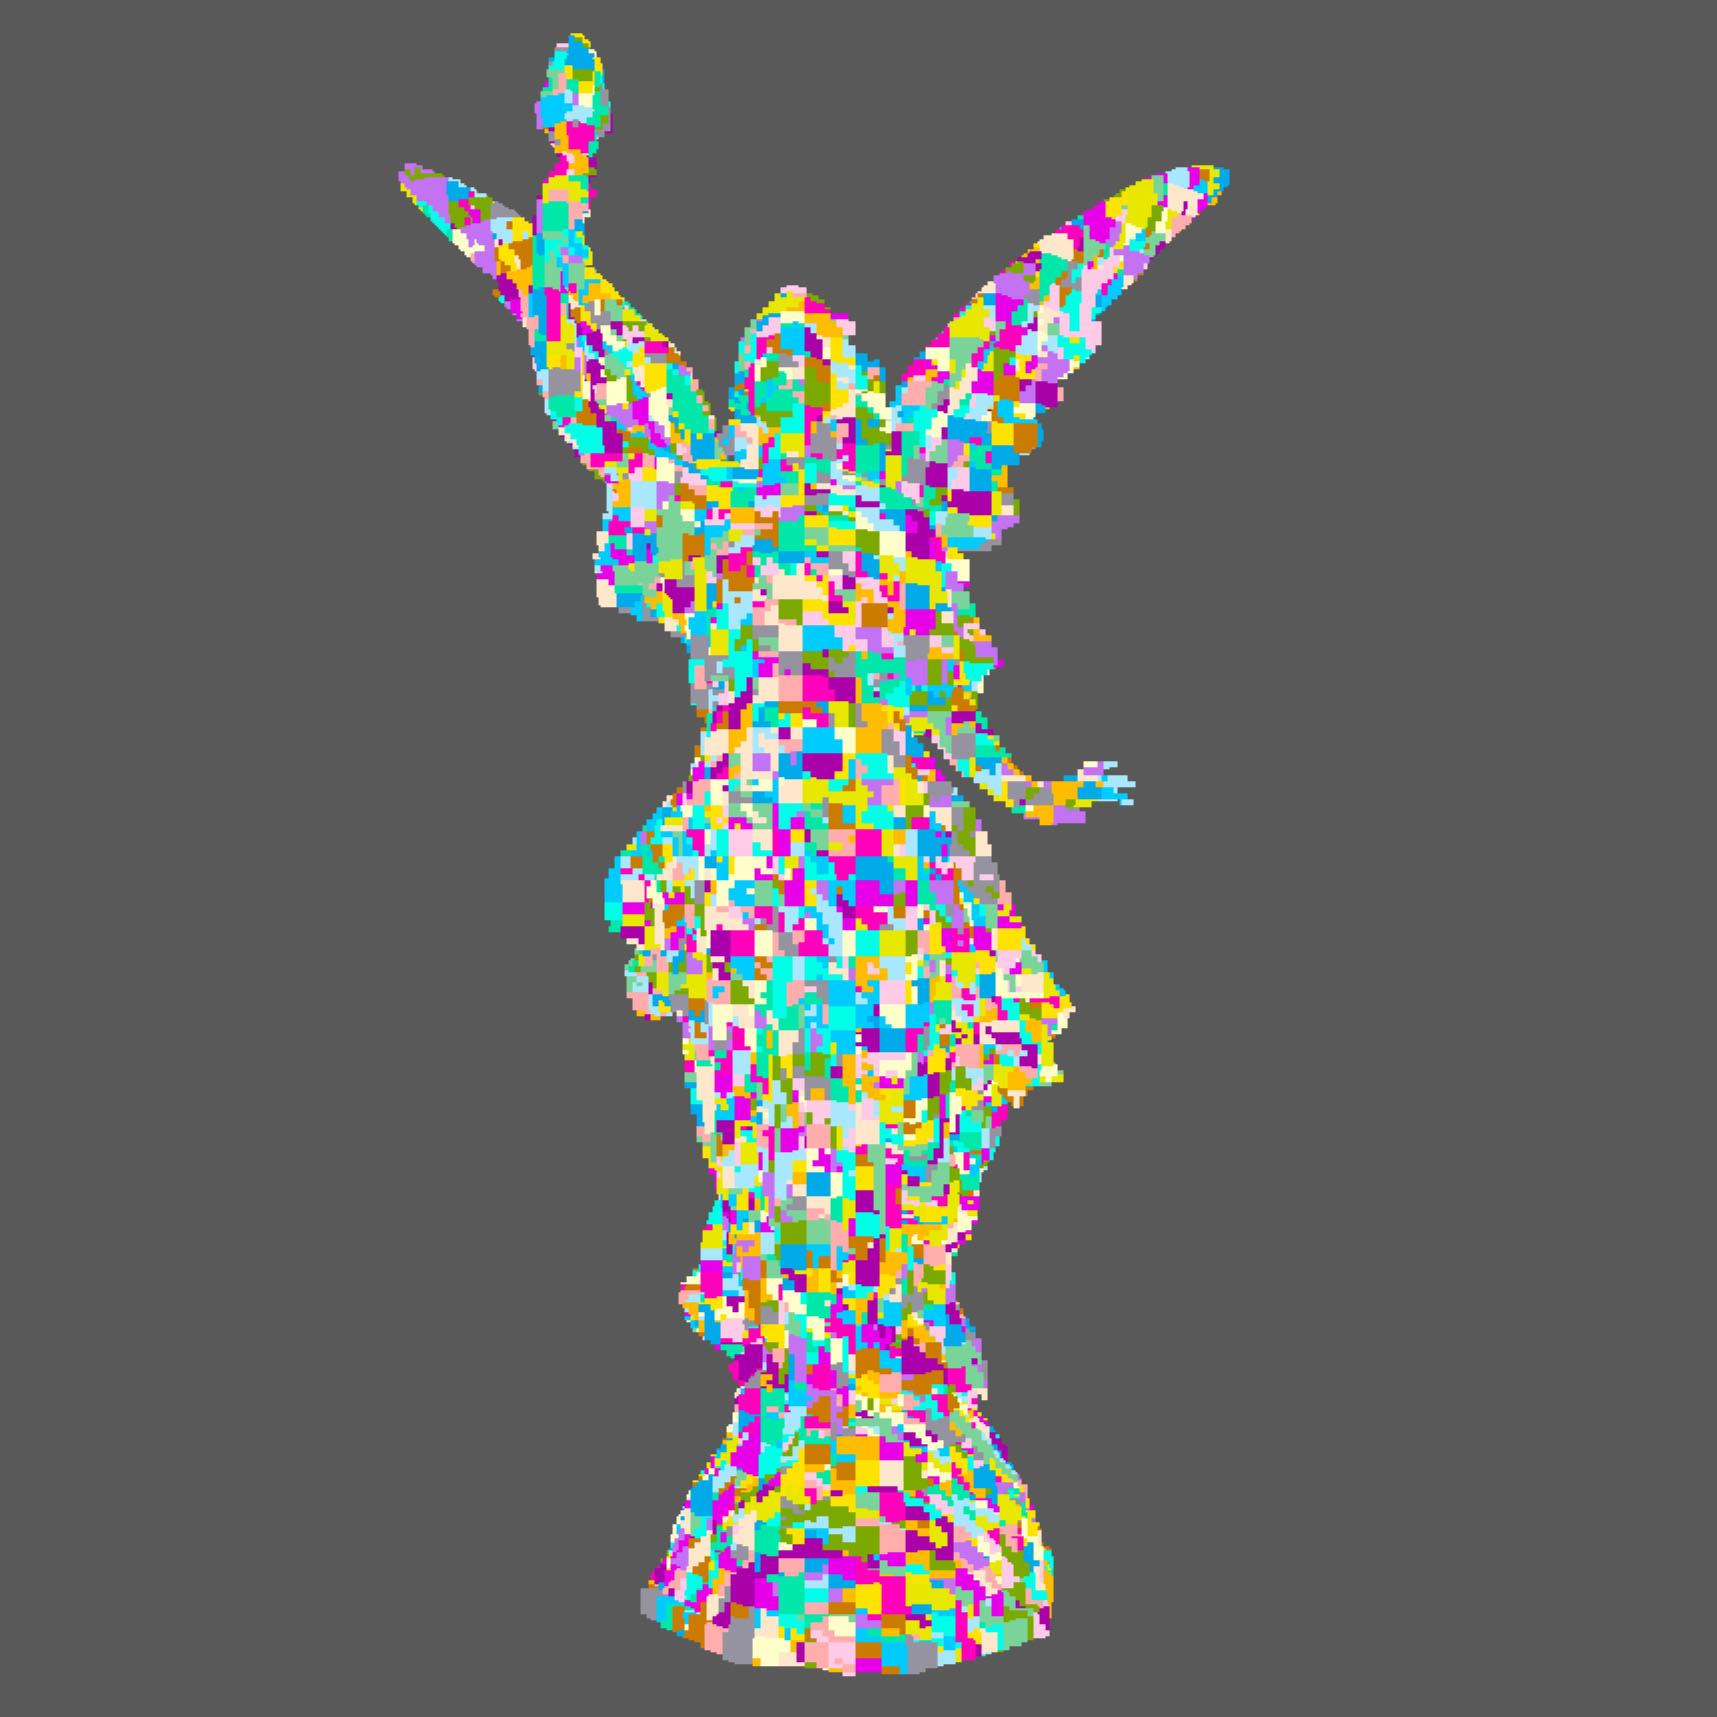
\includegraphics[width=151.5px]{images/graphics/lucy-voxel-octree-viz.jpg}
    
\includegraphics[width=250px]{images/graphics/lucy-voxel-octree-viz-2.jpg}
    \caption{The octree structure visualized. Each color represents one octree node. The whole model contains 
    \emph{470.355} voxels and \emph{19.823} octree nodes, with one octree node holding up to \begin{math} 5 \times 5 \times 5 \end{math}
    voxels.}
    \label{fig:voxel-octree-viz}
\end{figure}

\subsection*{Depth Pre-Pass}

The depth pre-pass now draws the best occluders to the depth buffer. To get a better understanding of what this 
means, figure \ref{fig:best-occluder-viz} shows the best occluders. Note, that the best occluders in this 
visualization are not hierarchically aggregated, which results in a slightly different visual result than what 
the actual depth buffer shows. 

\begin{figure}[h]
    \centering
    
\includegraphics[width=200px]{images/graphics/lucy-best-occluders-viz.jpg}
    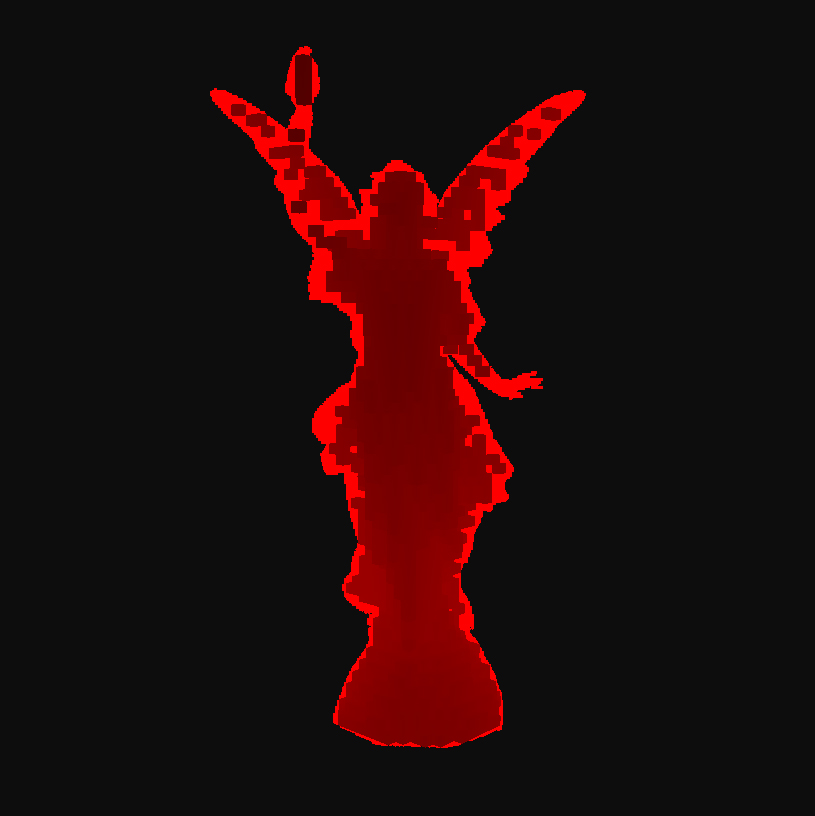
\includegraphics[width=200px]{images/graphics/lucy-best-occluders-diff-viz.jpg}
    \caption{A visualization of the best occluders (left) and the best occluders blended with a silhouette 
    of the whole voxel model. Each color represents one octree node which is considered to be a best occluder.
    The best occluders describe the non-visible core of the model and can be aggregated and used to occlude 
    many non-visible voxels during rendering.}
    \label{fig:best-occluder-viz}
\end{figure}

\noindent 
After drawing the best occluders to the depth buffer, it is copied into the \ac{HiZ} texture resource. 
Then the \ac{HiZ}-pyramid is constructed. This is done by a compute shader to optimize the work. The compute shader 
sequentially accesses the last valid mip level from mip level 0 to mip level \emph{n}, \emph{n} being the last 
mip level that is larger than a specified threshold. The compute shader accesses a grid of \begin{math} 2 \times 2 
\end{math} texels and takes the maximum value of all the 4 depth values. This maximum value is then stored in the 
subsequent mip map, then the next \begin{math} 2 \times 2 \end{math} texels are accessed. When all mip levels are 
constructed, the \ac{HiZ}-pyramid can be used for occlusion culling. \\

\noindent
The construction of the \ac{HiZ}-pyramid can possibly be further optimized by computing values for all mip levels 
in parallel, instead of sequentially writing and reading the values to or from a given mip level. 
The final \ac{HiZ}-pyramid is illustrated in figure \ref{fig:lucy-hiz-pyramid}.

\begin{figure}[h]
    \centering
    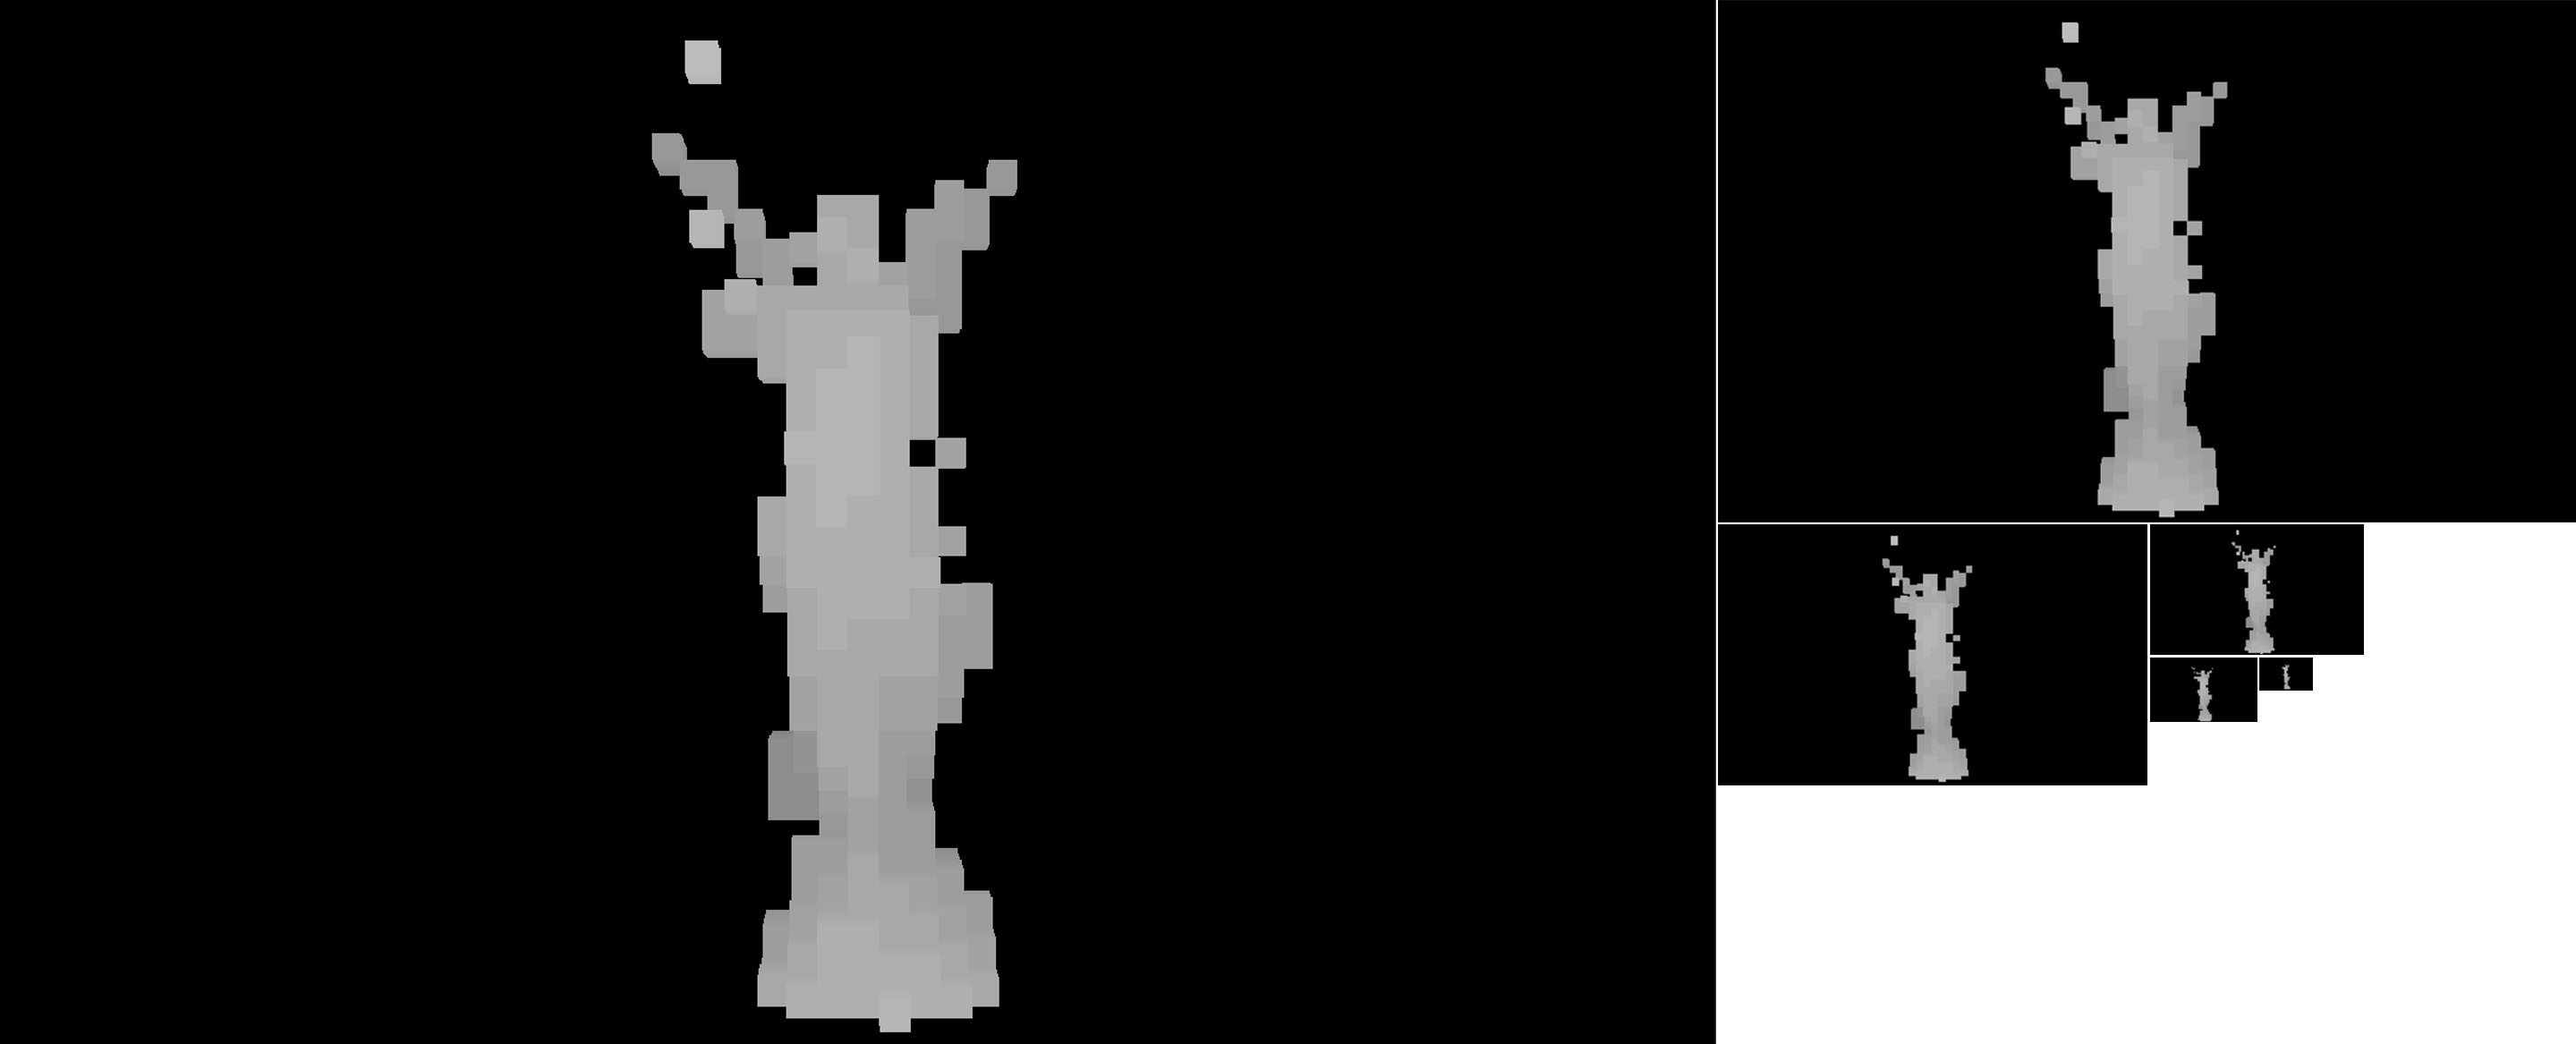
\includegraphics[width=\linewidth]{images/graphics/lucy-hiz-pyramid-inverted.jpg}
    \caption{The \ac{HiZ}-pyramid featuring the full resolution depth buffer as well as the individual mip map 
    levels. The color representation was inverted for better visualization.}
    \label{fig:lucy-hiz-pyramid}
\end{figure}

\subsection*{Culling and Draw Call}

The final draw call is initiated when dispatching the task shader. It accesses the \emph{voxel position buffer}, 
the \emph{octree node buffer} and the \emph{\ac{HiZ}-texture}. Each octree node is assigned to one threadgroup which will 
in turn compute one voxel (meshlet) per thread. The octree data just points to the relevant part of the voxel position buffer 
to get the position data. Each octree node is checked against the camera view frustum in order to cull it, if not visible.
Figure \ref{fig:lucy-frustum-culling} shows a partially culled model from a different perspective. 

[@TODO: Change model to stanford bunny!]
\begin{figure}[h]
    \centering
    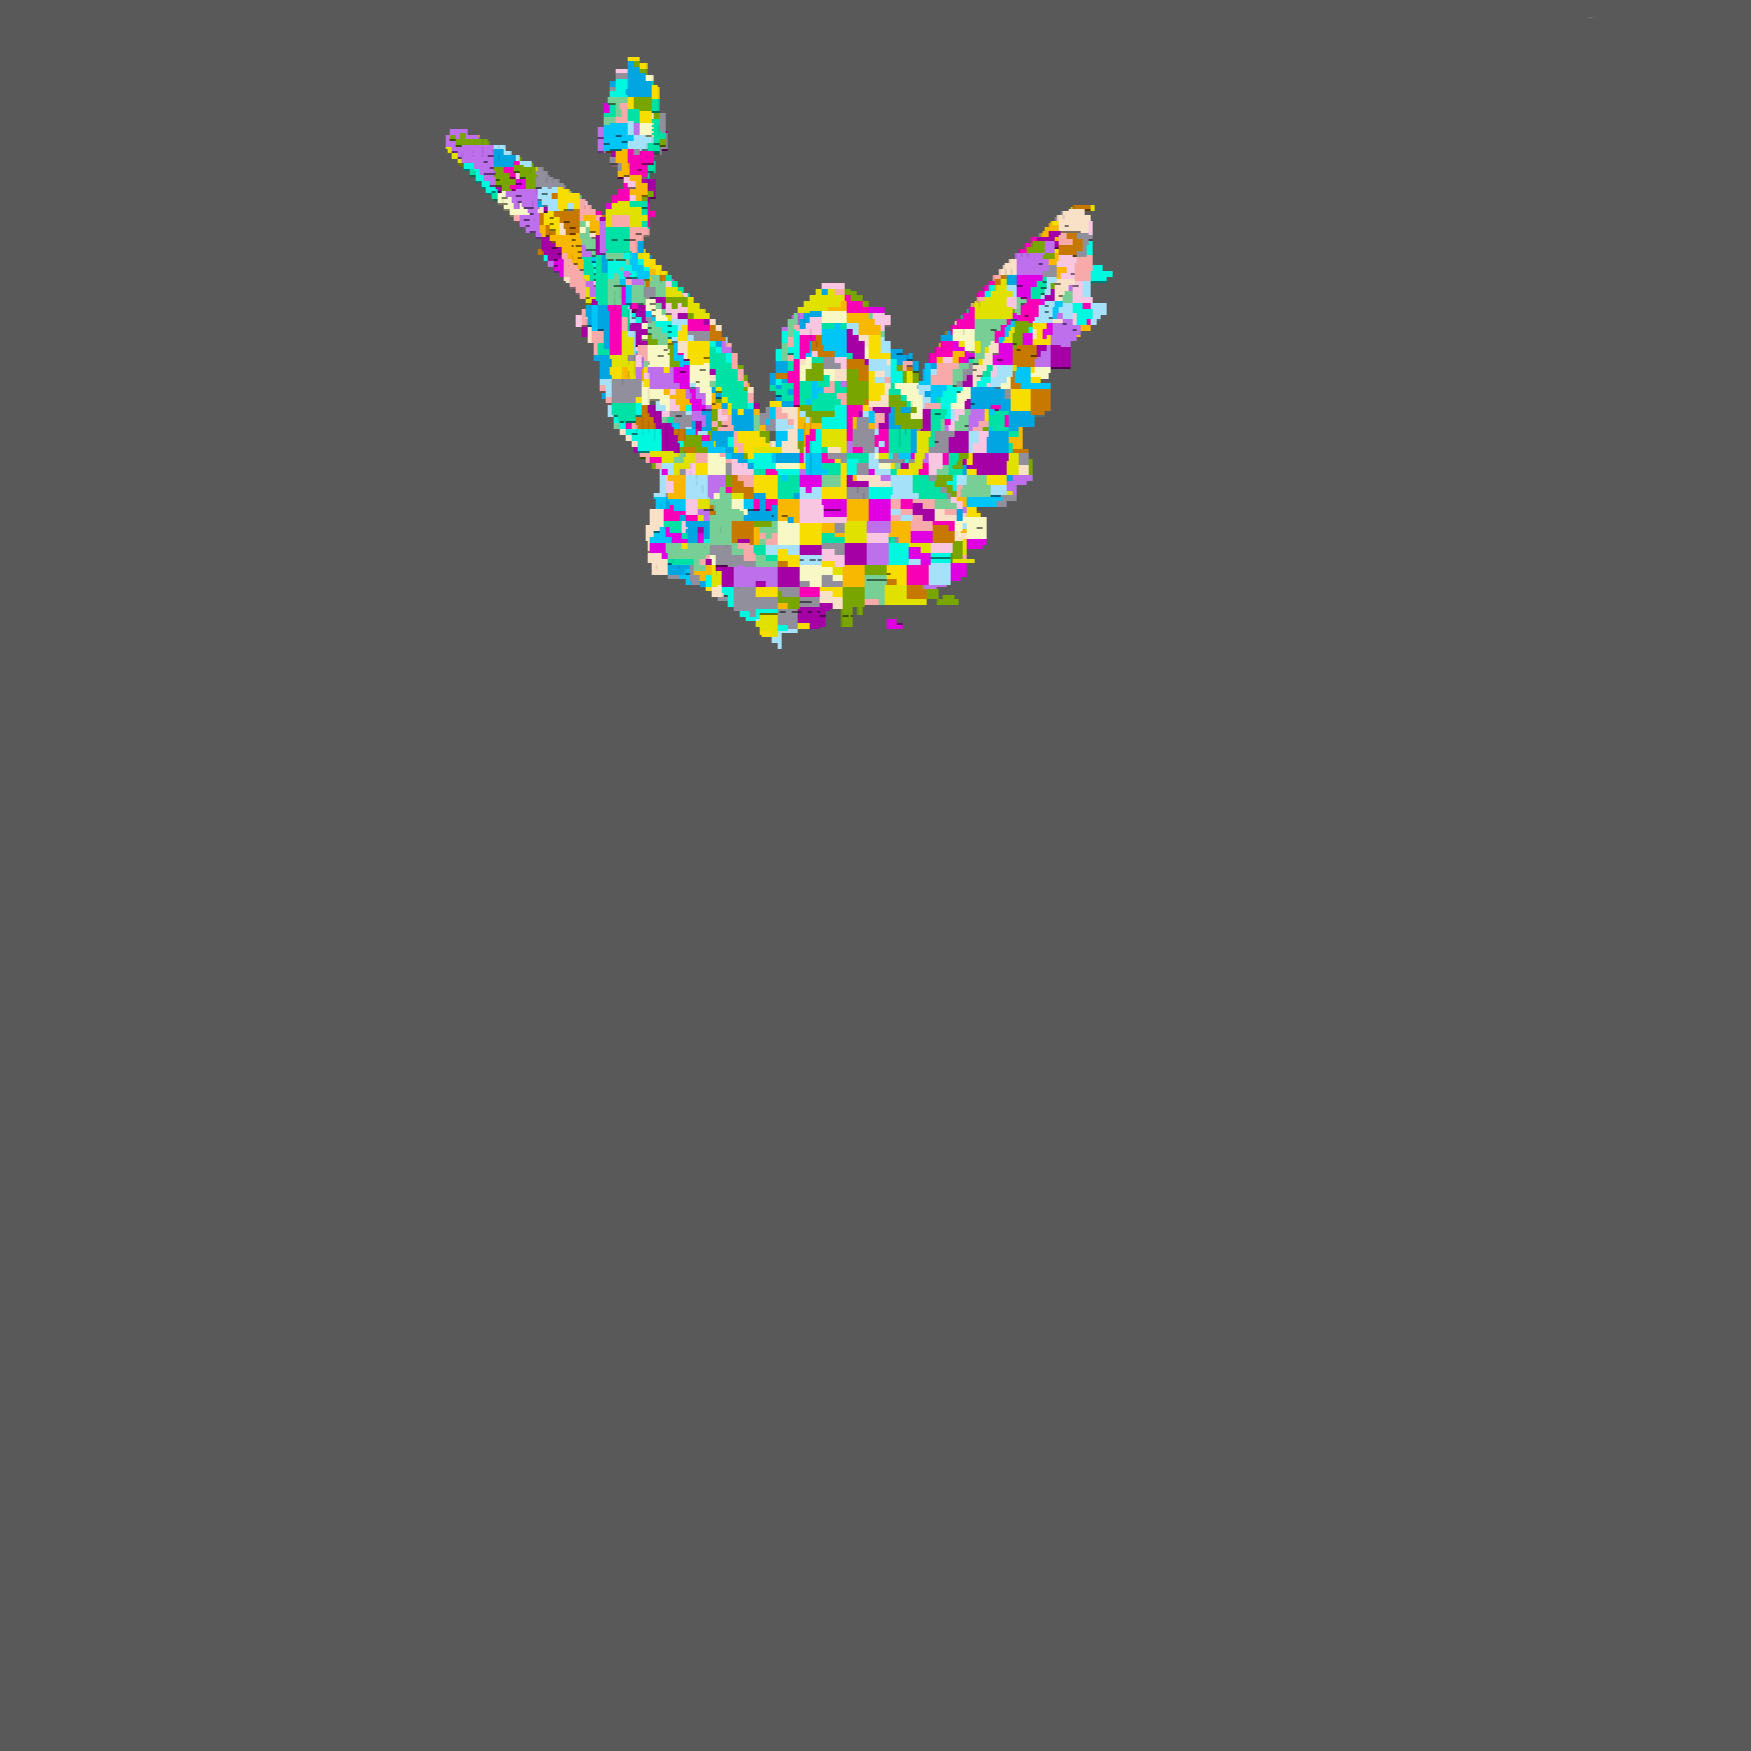
\includegraphics[width=200px]{images/graphics/lucy-frustum-culling.jpg}
    \caption{The whole \emph{Lucy} model culled against the view frustum. Octree nodes which are not visible are being 
    culled and are therefore not visible.}
    \label{fig:lucy-frustum-culling}
\end{figure}


\noindent [@TODO: Check if meshlets or octree nodes are culled in the end]
Non-culled nodes are then drawn, checking each voxel (meshlet) for occlusion against the \ac{HiZ}-texture and its mip maps. 
This operation introduces additional overhead which is normal for any acceleration struture. The goal is always to apply it 
to a scenario, where the additional overhead is compensated by the acceleration it provides. In this case, the visible voxels 
might have to pass the whole \ac{HiZ} structure. The non-visible voxels, however, will likely early-exit after just a few 
operations, comparing against the mip map hierarchy. In a volumetric representation, the candidates for non-visible voxels 
are plenty, as usually, only a fraction of the voxel data needs to be drawn at any time. Essentially, all voxels, but the 
outer, visible layer, can be omitted.\\

\noindent
The voxels that passed all tests are finally dispatched for the final draw call, keeping the memory bandwidth to a minimum, 
since the geometry, UVs, normals and more can be easily created on-chip. \\


\section{Occlusion Culling Algorithm} \label{sec-occlusion}

The occlusion culling algorithm is the central part of the pipeline and thus deserves a more detailed coverage. The 
basic implementation is very similar to the ones provided by Aaltonen et al., Greene et al. or Karis et al. 
\cite{Aaltonen2015,Greene93,Karis2021}. It relies on the pre-computations discussed above and can be applied to the 
octree nodes or to individual meshlets. Usually, octree nodes are culled in this process, as \cite{AkenineMoeller2018}
points out. However, using the mesh shading pipeline it has become possible to cull more fine granular by using 
meshlet bounding volumes as occludees. One advantage is that geometry can be culled, even when the occluder doesn't 
fully overlap the octree node. Therefore, even small instances in the scene can occlude a lot of geometry, resulting 
in better performance overall. On the other hand, this approach requires a lot more computations because all meshlets 
are checked against the \ac{HiZ}-pyramid. Eventually, it is necessary to make precise measurements in order to find out 
which approach works best under the given circumstances. In general, it is hard to predict the performance of 
parallelized \ac{GPU} computations. For this implementation the culling of octree nodes is assumed. 

\subsection*{Visibility Computation} \label{subsec-visibility-computation}

As mentioned before, the task shader is used to pre-select and pre-process the scheduled geometry data, 
which in this case is just the position of an individual octree node and all the voxels (meshlets) inside of the 
node. This precomputational step is used for visibility checking, i.e. view frustum culling and occlusion culling. 
Since the task shader is just a general term for any compute shader used before dispatching the meshes, 
this pipeline step is realized using the standard compute architecture. \\

\noindent
To ceck for visibility, \emph{projected bounding boxes} need to be constructed and checked against the 
\ac{HiZ}-pyramid. This step can be highly parallelized by using one \ac{GPU} thread per bounding box calculation. 
The first step involves the projection of the bounding box onto the view plane, which results in a clip space 
representation of the data. This early projection is done for all eight vertices of the bouding box, so the minimum 
and maximum values on each axis can be calculated to end up with clip space and eventually with screen space coordinates.
The min and max values for each axis represent a screen space rectangle, which can be used for the depth test. The 
rectangle has the following characteristics.

\begin{itemize}
    \item The minimum and maximum \emph{x} values describe the \emph{width} of the rectangle.
    \item The minimum and maximum \emph{y} values describe the \emph{height} of the rectangle.
    \item The minimum \emph{z} value describes the \emph{depth} of the rectangle, i.e. nearest vertex of the bounding box.
    \item The minimum and maximum \emph{x} and \emph{y} values describe the \emph{position} of the rectangle in clip space.
\end{itemize}

\noindent [@TODO: Add image of this!]
The rectangle can be transformed into screen space and can be expressed as UV coordinates for sampling the 
\ac{HiZ}-pyramid. To check for visibility, all vertices are assumed to be at the same distance from the camera,
i.e. to have the same depth value. This depth value is the minimum \emph{z} value calculated earlier. This way,
as long as any vertex of the rectangle is located \emph{in front} of the best occluders stored in the 
\ac{HiZ}-pyramid, the rectangle could be visible partially or completely. Conversely, as long as all vertices of 
the rectangle are located behind the best occluder, the rectangle must be completely occluded. A visualization of 
this process is shown in figure \ref{fig:screen-space-occlusion-test}.

\begin{figure}[h]
    \centering
    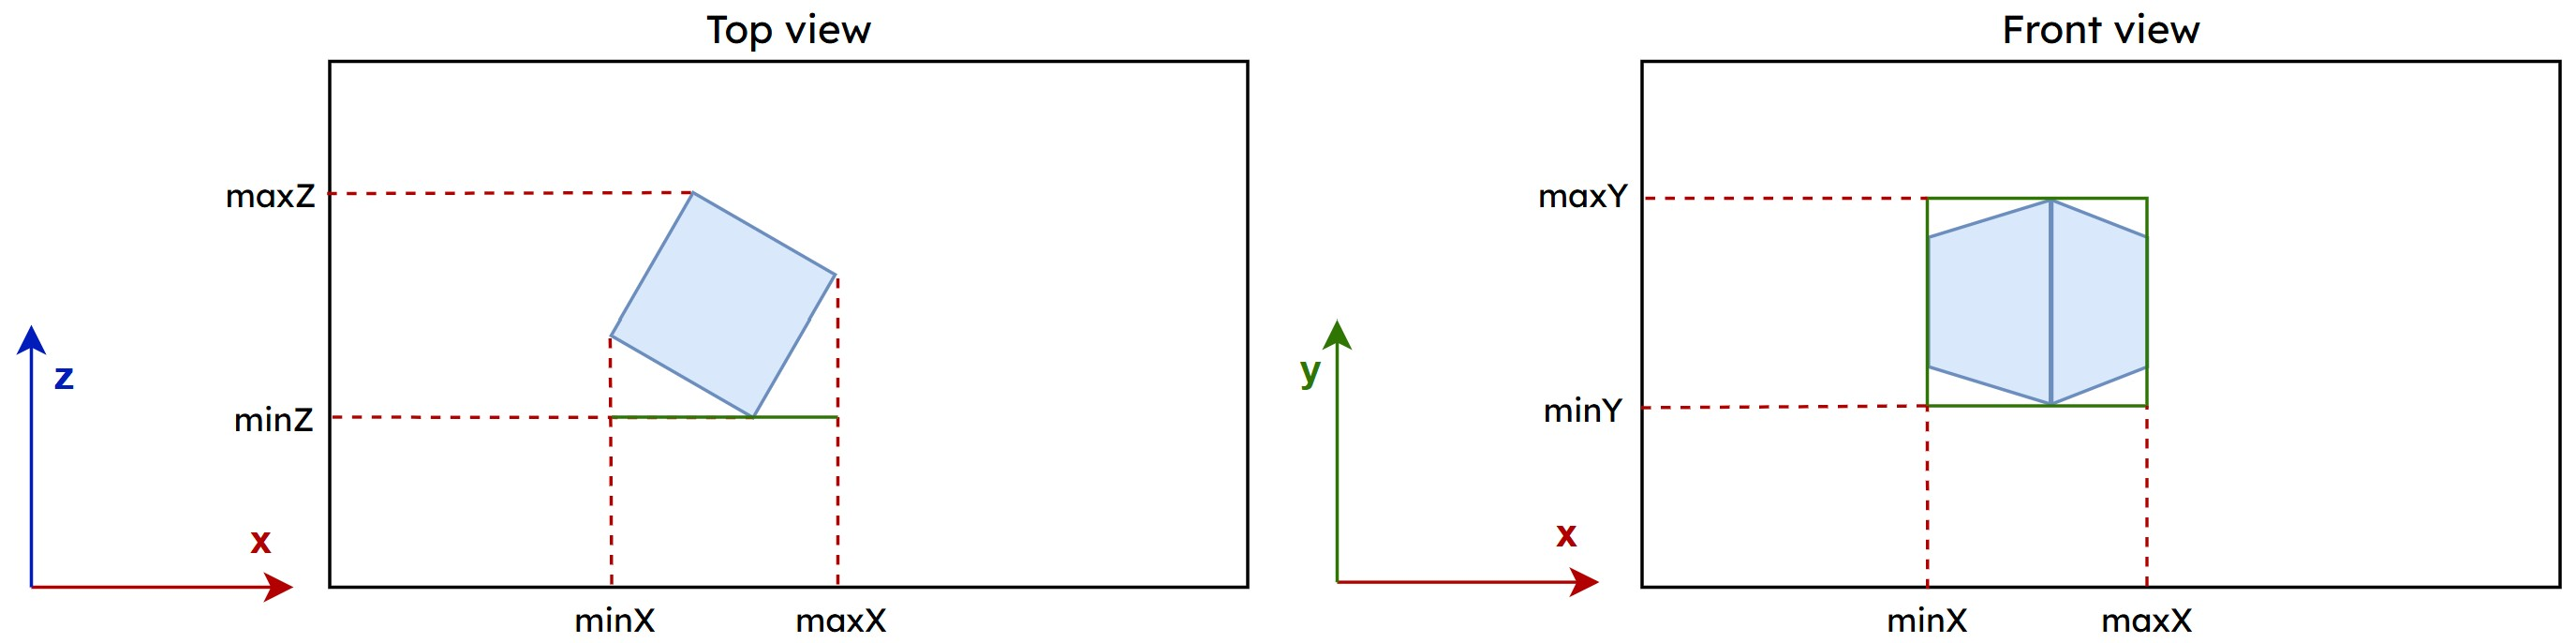
\includegraphics[width=\linewidth]{images/graphics/screen_space_occlusion_test.jpg}
    \caption{The occlusion test is done in screen space using the minimum and maximum boundaries. The octree node 
    is shown in blue, and the respective minimum and maximum values are traced by the dotted red lines. The green 
    line represents the rectangle as viewed from above (left). The same rectangle is shown from a front view as a 
    representation of the octree nodes screen space occupancy (right).}
    \label{fig:screen-space-occlusion-test}
\end{figure}

\noindent
The rectangles corners can now be used as coordinates for sampling the \ac{HiZ}-pyramid. Since the minimum \emph{z} 
value is used for all corners, the rectangle describes a flat plane in the clip space. It is sufficient for the 
depth testing to sample the four corners and compare each depth value sampled from the pyramid to the minimum \emph{z},
as shown in figure \ref{fig:visibility-hiz-sampling}.
In fact, it is sufficient to compare the lowest of the four \emph{z} values to the minimum \emph{z} value. Now the 
hierarchy is traversed until the node is found to be fully occluded or until the hierarchy is fully traversed and the 
node is found to be visible. Note, that the area which is checked is not perfectly congruent with the actual projected 
boundary box. This can lead to edge cases, where a few percent of the octree nodes are drawn although they are actually 
completely occluded.

\begin{figure}[h]
    \centering
    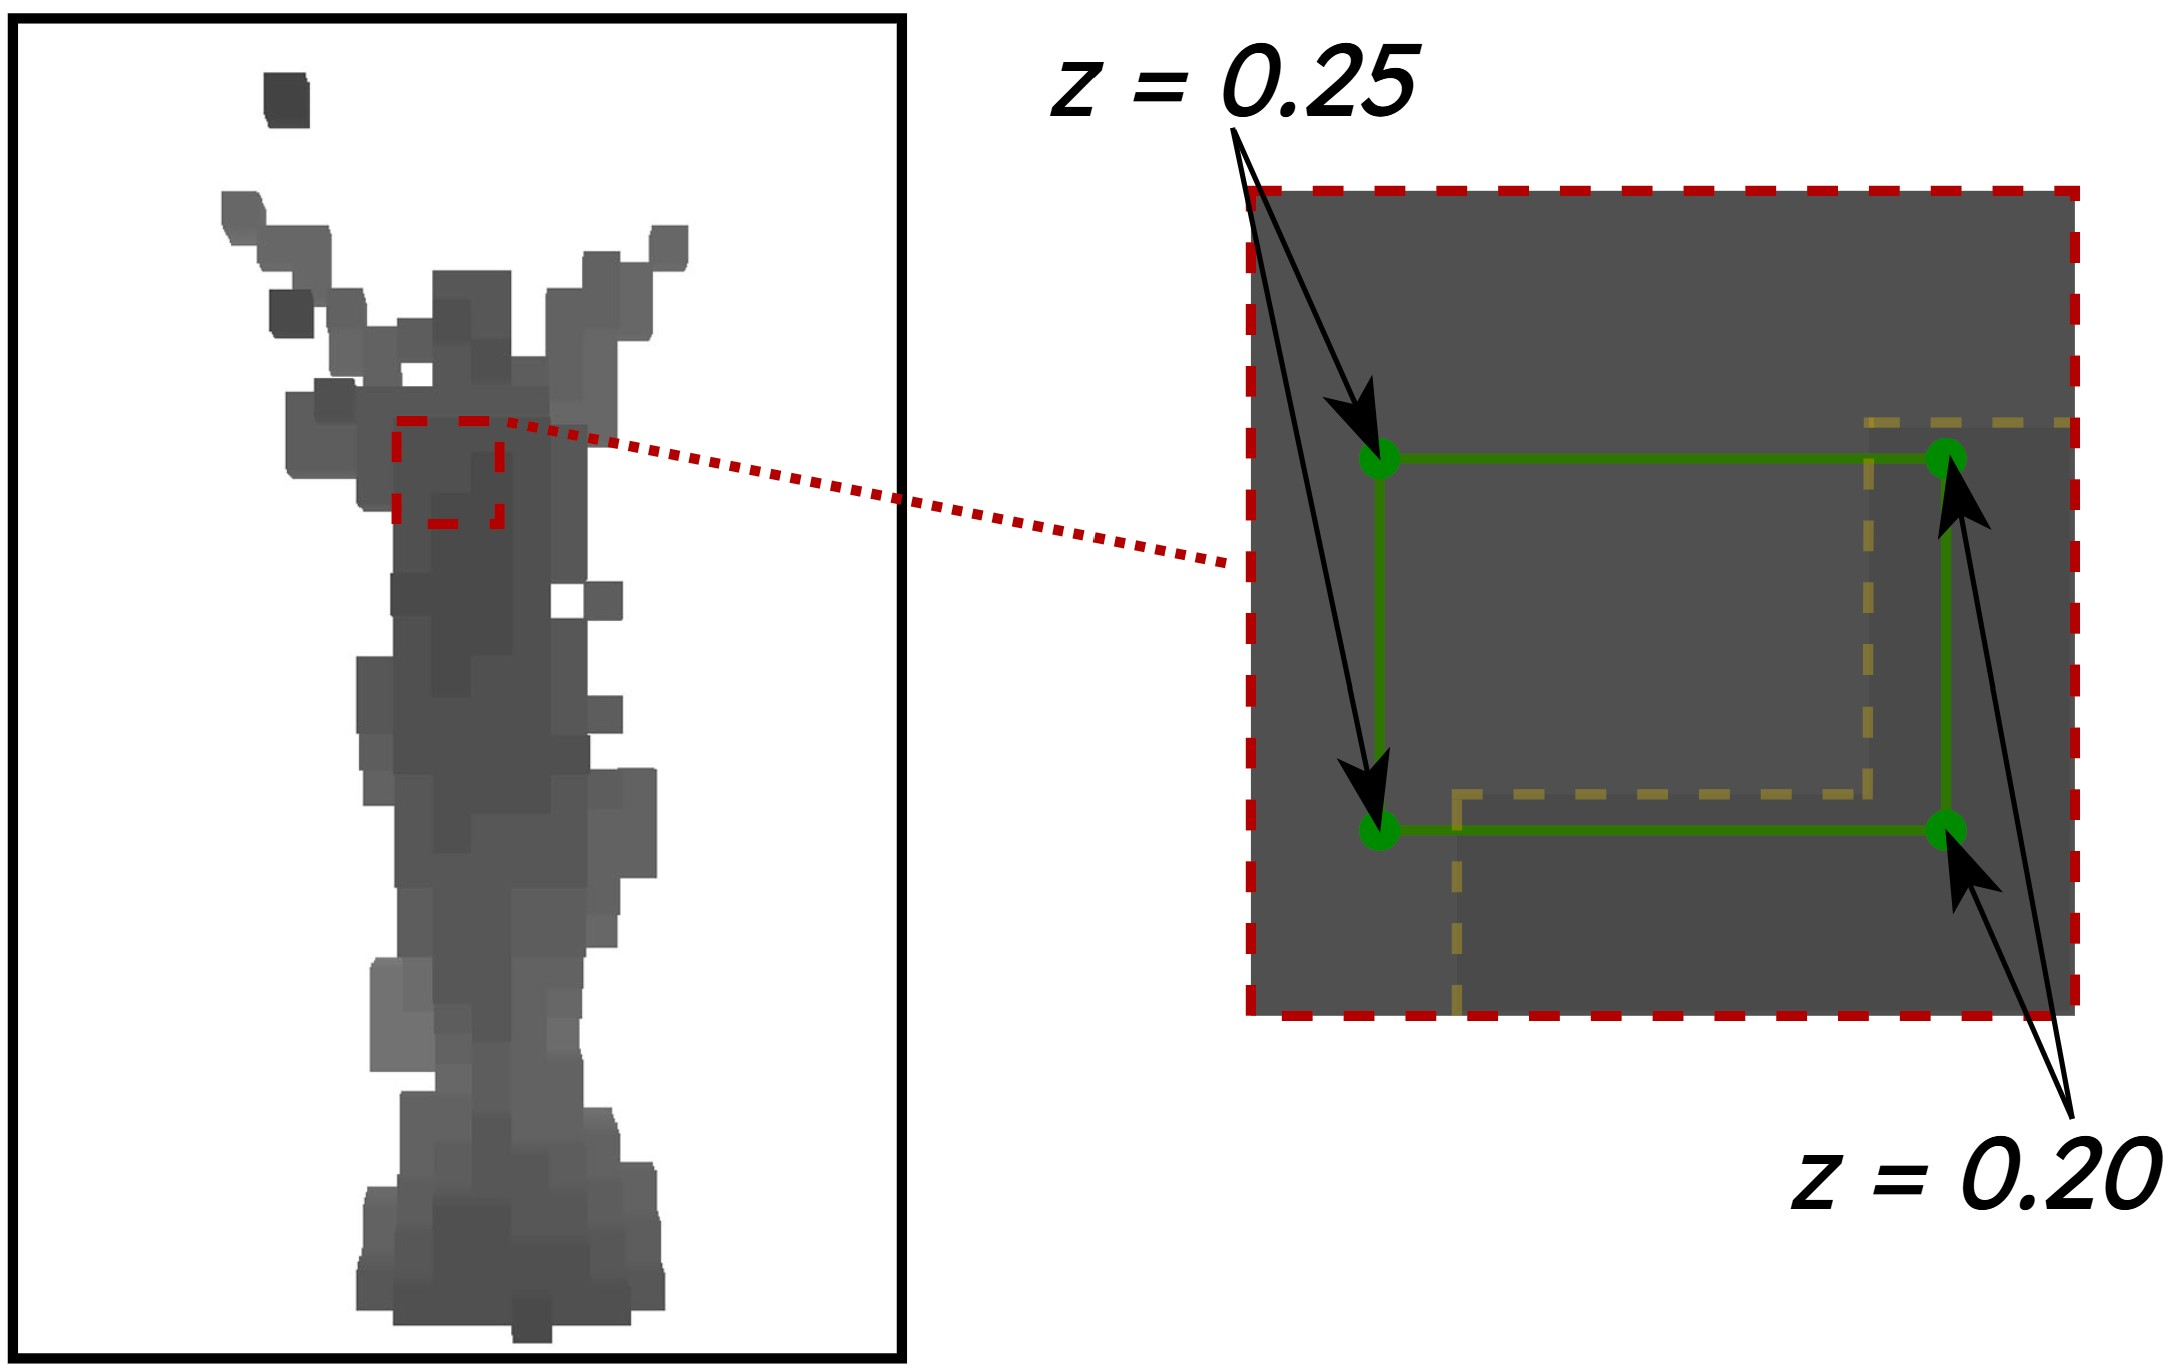
\includegraphics[width=\linewidth]{images/graphics/visibility-hiz-sampling.jpg}
    \caption{The \ac{HiZ}-pyramid being sampled using the vertices of the screen-space rectangle, shown in green. 
    The dotted yellow line resembles the border between different depth values in the buffer. Sampling the four 
    vertices can provide up to four different depth values. The smallest one being the "nearest" occluder.}
    \label{fig:visibility-hiz-sampling}
\end{figure}


\noindent
The complete occlusion culling routine computes the bounding box vertices as \emph{uv} coordinates so it is independent 
from the mip level the depth values are checked against. In the best case scenario, the visibility can be determined in 
using the coarsest mip level. In the worst case, all mip levels up to the full resolution depth buffer need to be checked.
The routine is shown in listing \ref{lst-occlusion-culling-algo} as pseudo code.

\fbox{
\begin{minipage}{\linewidth}
\begin{algorithm}[H]
\SetAlgoLined
\KwIn{float4 basePosAndScale}
\KwResult{Boolean indicating whether a bounding box is visible}

\SetKwFunction{FMain}{IsVisible}
\SetKwProg{Fn}{Function}{:}{}
\Fn{\FMain{float4 basePosAndScale, Texture2D HiZPyramid}}
{
    float4 center $\gets$ float4(basePosAndScale.xyz, 1.0f)\;
    float scale $\gets$ abs(basePosAndScale.w)\;
    \BlankLine

    float minX $\gets$ GetMinXFromProjectedBoundingBox(center, scale)\;
    float maxX $\gets$ GetMaxXFromProjectedBoundingBox(center, scale)\;
    float minY $\gets$ GetMinYFromProjectedBoundingBox(center, scale)\;
    float maxY $\gets$ GetMaxYFromProjectedBoundingBox(center, scale)\;
    float minZ $\gets$ GetMinZFromProjectedBoundingBox(center, scale)\;
    \BlankLine

    rect uvRect $\gets$ CalculateUVRect(minX, maxX, minY, maxY, minZ)\;
    \BlankLine

    \For{$mipLevel \gets HiZPyramid.GetNumMipLevels() - 1$ \KwTo $0$}{
        float depthVertex1 $\gets$ HiZPyramid.Sample(uvRect.vertex1, mipLevel)\;
        float depthVertex2 $\gets$ HiZPyramid.Sample(uvRect.vertex2, mipLevel)\;
        float depthVertex3 $\gets$ HiZPyramid.Sample(uvRect.vertex3, mipLevel)\;
        float depthVertex4 $\gets$ HiZPyramid.Sample(uvRect.vertex4, mipLevel)\;
        \BlankLine

        \If{max(depthVertex1, depthVertex2, depthVertex3, depthVertex4) < minZ}{
            \Return{false}\;
        }
    }

    \Return{true}\;
}
\caption{Occlusion Culling algorithm.}
\label{lst-occlusion-culling-algo}
\end{algorithm}
\end{minipage}
}
    
\vspace{0.5cm}



[@TODO: Mention view frustum culling in depth pre pass]
[@TODO: Check if I should explain mip levels in chptr 4]


// --------------------------------------------------------------------------------- //
Motivation:
Use Meshlet Culling in voxel rendering to optimize GPU Driven Voxel Rendering

- Where can I put the initial thought of having voxels as meshlets? -> maybe motivation? 
- Early-z rejection vs. our approach

Implementation Considerations:

- Meshlet Culling at first, then problem, because meshlet culling algorithm depends on different algos
    - Meshlet Backface Culling -> Not possible because Meshlets are voxels in this case
    - Meshlet Occlusion Culling -> Using 2 Pass Depth Occlusion Culling sounds good!
    - 2PDOC relies on drawing best occluders which are usually hand picked by artists (buildings)
        -> We can dynamically pick best occluders by selecting full octree nodes as best occluders!

- [x] Optimize octree by using High Res SVOs (https://www.cse.chalmers.se/~uffe/HighResolutionSparseVoxelDAGs.pdf).
    - As shown in the paper, here we also only need to encode if a node is filled or not. This way we can 
    optimize memory and proccessing speed! (Not done here because of limitation in loading and voxelizing models.)

- Explain why Mesh Shading is useful here and what the differences to HiZ and Two-Pass OC are!

- Consider further optimization by removing redundant computations (e.g. for HiZ depth test, meshlets (or octree nodes)
are already projected to screen space. This is then done again in the mesh shader. Maybe it could be an optimization 
to do the projection in the task shader already, so it is only computed once. The already projected position 
could then be input in the mesh shader, making the projection in the mesh shader redundant).

- Why not just discard octree nodes when I already know that they are not visible. -> Because they could as well be the
  surface of the model! + can be used as occluders for rest of the scene

- Limitations: 
    - Worse performance on slopes? -> Check and measure!
    - Align octree bounds with outer most voxel bounds, so no misalignment happens!

    - (Larger nodes which are not being split can be "full" without being full!)

// --------------------------------------------------------------------------------- //
